\chapter{Alignment of the SciFi}
\label{sec:story}

% I'd like you to think about the work you have been doing on the alignment and what things have been investigated and what conclusions you have made. You want to build the story one piece at a time, so I think it will start with testing some of the constraints from the null tests and going from there. With the type of work you have been doing, you will also have a much larger "future work" and "continuing work" section, I would put it before the conclusion. This will be discussing things like the way we discovered the cluster bias and the way that it is linked to the rotational degrees of freedom, etc. And it can outline the things you know about the way the real detector will be aligned starting very soon.

% \begin{itemize}
%   \item testing some of the constraints from the null tests
%   \item future work: discovered cluster bias + link to rotational degrees of freedom
% \end{itemize}

% taking notes for now so i know what plots to use
% \begin{enumerate}
%   \item started with null tests.
%   \item which constraint does what?
%   \item which degree of freedom moves what part of the scifi?
% \end{enumerate}

The alignment was performed using tracks and vertices. The alignables are the stations,
layers and modules.
The goal is to find the optimal configuration of constraints and degrees of freedom to align the detector to its physical position.
The following pre-installed alignment conditions with the survey constraints being\\
\\
"FT : 0 0 0 0 0 0 : 1 1 1 0.0003 0.0003 0.0003”\\
"FT/T. : 0 0 0 0 0 0 : 1 1 1 0.0003 0.0003 0.0003”\\
"FT/T./Layer(X1|U|V|X2) : 0 0 0 0 0 0 : 0.2 0.2 0.2 0.0001 0.0001 0.0001”\\
"FT/.*Module. : 0 0 0 0 0 0 : 0.1 0.1 0.1 0.001 0.001 0.001"\\
"FT/.*Mat. : 0 0 0 0 0 0 : 0.05 0.05 0.05 0.1 0.1 0.1”\\

were used.

The string is the name of the element, the first set of six numbers are hardcoded parameters for each of the 3 translation degrees of freedom and 3 rotational degrees of freedom (Tx, Ty, Tz, Rx, Ry, Rz) and the second set of six parameters are the corresponding uncertainties.

The scale for the translations are $\si{\milli\metre}$ and the scale for the rotations being $\si{\radian}$. A survey uncertainty of $\num{0.0001}$ stands for $\SI{0.1}{\milli\radian}$.

The alignment runs were performed with gaudisplititer.

During the alignment, lagrange constraints can be utilized to minimize the
$\chi^2$ under the condition
\begin{equation}
  f(\alpha) = 0
\end{equation}
and adding the lagrange parameter $\lambda$ to get
\begin{equation}
  \Delta \chi^2 = \lambda f(\alpha)
\end{equation}\,.

Lagrange constraints are added to fix losely constrained degrees of freedom and can be used for any linear combination of translations and rotations.

%include table from https://twiki.cern.ch/twiki/bin/view/LHCb/TAlignmentManual.

\section{Nulltests and software tests}

As a starting point, Alignment v17r1 was used with 5000 events, magnet in upward position and \textit{GoodLongTracks}.
The \textit{GoodLongTracks} have the following cuts and parameters:
\begin{itemize}
  \item minimum $P_{\text{total}} = \SI{5000}{\mega\electronvolt}$ %(units? 5000 MeV?)
  \item maximum $P_{\text{total}} = \SI{200000}{\mega\electronvolt}$ %(units? 200 000 MeV = 200 GeV?)
  \item minimum $p_T = \SI{200}{\mega\electronvolt}$ %(units?)
  \item maximum $\chi^2 = 5$
  \item track type should be categorized as "long" %(what does that mean -> hits in every subdetector)
%\item maximum number of THoles? is 1
\end{itemize}

and for the later used \textit{HighMomentumTTracks} the cuts and parameters are:

\begin{itemize}
  \item minimum $P_{\text{total}} = \SI{50000}{\mega\electronvolt}$
  \item track type should be categorized as "TTrack"
  \item maximum $\chi^2 = 5$
\end{itemize}

\begin{figure}
  \centering
  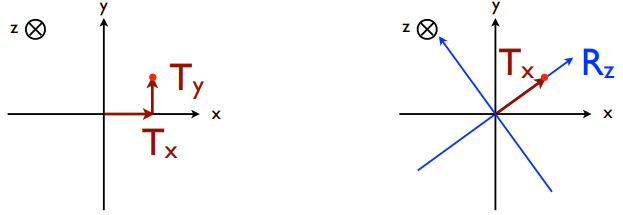
\includegraphics{plots/point_dofs.png}
  \caption{Different ways of describing a measurement point inside the detector.}
  \label{fig:dofs}
\end{figure}

At first, a series of tests regarding different degrees of freedom and lagrange constraints is performed to find the optimal solution for the SciFi.

The real detector layers are all centered around the beam pipe with no shifting
in any direction and the goal is to align the layers in the software to mirror
the real layers and reduce the shifting as close to zero as possible.

Figure \ref{fig:dofs} is used to demonstrate which degrees of freedom can be used
to describe a point in the detector or a shift in coordinates.
On the left-hand side the measurement point is described through cartesian coordinates and on the right-hand side it is described via polarcoordinates in a way.

As a baseline the configuration from Florian Reiss is used.
The degrees of freedom used by florian are $Tx$ and $Rz$ and he did not use any constraints so what we compare to is an unconstrained detector. He used \textit{GoodLongTracks} and aligned the stations and layers.
In this part, the steps of testing different configurations is described and analysed.
%What is florians configuration?? -> lxplus, one of the first plots.

The measurement points are the mean of each layer, the errorbars are root-mean-square errors and come from the difference between the C-side and the A-side of the detector layer and is not the measurement uncertainty.
The green measurement used the following configuration:

\begin{itemize}
  \item 1000 events
  \item GoodLongTracks
  \item degrees of freedom: Tx Tz Rx Rz
  \item constraints:
  \begin{itemize}
    \item station3 : Tx Tz Rx Rz
    \item last C-frame : Tx Tz Rx Rz
  \end{itemize}
\end{itemize}

At first i used every degree of freedom except for $y$-translation and rotation. Although there is a redundancy in information it helps to not lose information. Later on we want as few constraints as possible and only usefull degrees of freedom, so we started with a lot of constraints and degrees of freedom and reduce them as we procede. This measurement only used 1000 events and is only used as a guideline to what the trend of the distribution looks like. The associated graphs for $Tx$ plotted against the group position in $z$ are shown in figure \ref{fig:june_2}.
A prominent problem we see in the blue graph is the layer separation between the X-layers and
the stereo layers. This is definitely not how the physical detector is mounted so this is the baseline we want to align.
The green dots from the first alignment run with 10 iterations looks promising
but we only used 1000 events so this result only shows a trend how good the alignment worked.

\begin{figure}
  \centering
  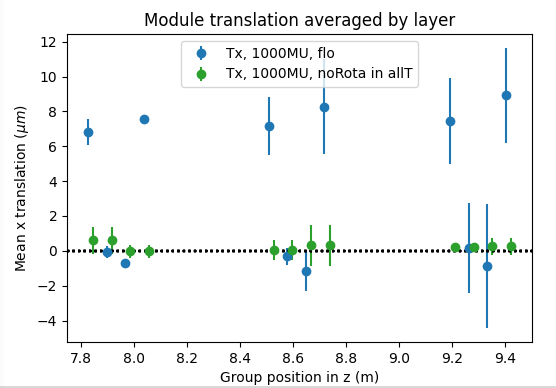
\includegraphics[width=0.8\textwidth]{plots/june_21/Tx_noRota_allT_1000MU.png}
  \caption{comparison of different configurations without rotational constraints in every station, magnet up and 1000 events. plotted is translation in x versus global z.}
  \label{fig:june_2}
\end{figure}

\begin{figure}
  \centering
  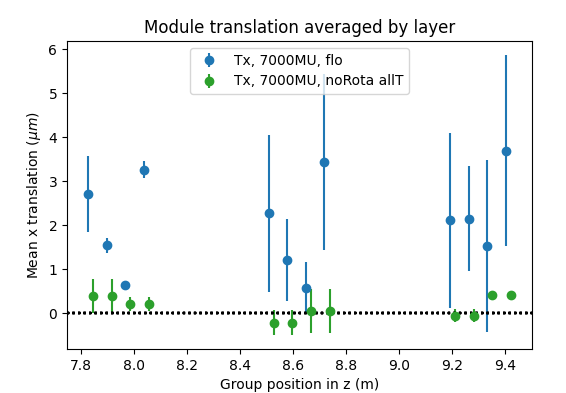
\includegraphics[width=0.8\textwidth]{plots/june_21/Tx_noRota_allT_7000MU.png}
  \caption{comparison of different configurations without rotational constraints in all stations, magnet up and 7000 events. plotted is x translation versus global z.}
  \label{fig:june_2_1}
\end{figure}

In figure \ref{fig:june_2_1} the same measurement was performed for 7000 events to get a better picture. In comparison to \ref{fig:june_2} an overall improvement in Florians configuration is visible and the layer-splitting is reduced but still prominent. The green measurement shows no direct improvement since the layers are already pretty close to zero in x-direction, where we want them.
Here we studied the impact of not constraining rotations which worked quite good.

The following measurements used 3000 events because the performance did not change much when using 5000 or even 7000 events. Also, the time the computer needed to finish an alignment run for 7000 events and 10 iterations was a lot longer than for 3000 events.
This alignment took 9 iterations to converge so there is also a computing error
which needs to be sorted out.

A clear evidence of this computing error can be seen in figure \ref{fig:june_3}. Here a comparison between a modified configuration from florian shown in the blue dots, and a new configuration using halflayer constraints shown with the orange dots, is performed.
This new configuration in orange converged after 15 iterations which is not what we want since the alignment will be done with many more events and this would take too much time if there was this error.

\begin{figure}
  \centering
  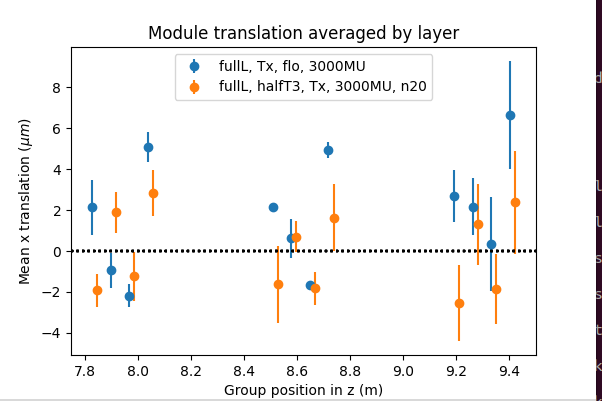
\includegraphics[width=0.8\textwidth]{plots/june_21/allT_halfT3_n20_Tx.png}
  \caption{analysed 20 iterations for x translation behavior (look up exact constraints and dofs)}
  \label{fig:june_3}
\end{figure}

\begin{figure}
  \centering
  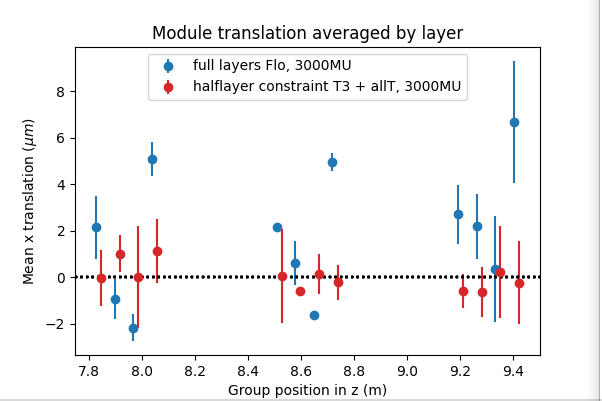
\includegraphics[width=0.8\textwidth]{plots/june_21/allT_halfT3_Tx_vs_Flo.png}
  \caption{halflayer constraints and full layer constraint, very strict (look up exact constraints and dofs)}
  \label{fig:june_4}
\end{figure}

The consequences of very strict Tx constraints are shown in figure \ref{fig:june_4}.
The difference between the configuration used here and the one used in figure
\ref{fig:june_2_1} are... (comparison todo).

Introducing halflayers as an alignable, they are constrained in station 3 because
we found that it results in the best alignment.
Also halflayers are a better representation of the real detector since we describe
the C-side and A-side seperately.
This is due to the fact that station 3 is the furthest away from the interaction point (IP) and $q \,/\, p$ has the most impact at that distance.
Looking at $Tz$ first, the RMS uncertainty is viewed by looking at the A-side and the C-side seperately.
A clear layer separation is visible in terms af layer translation along the beam pipe\ref{fig:june_5}.
The first and third layer in each station move away from the IP and the second and
fourth layer move away from the IP.
Because of the many constraints that are applied to T3, the RMS uncertainty in the other stations get worse. Because the last station is overconstrained the track reconstruction moves the other stations accordingly which results and larger RMS uncertainty in station 1 and 2.

\begin{figure}
  \centering
  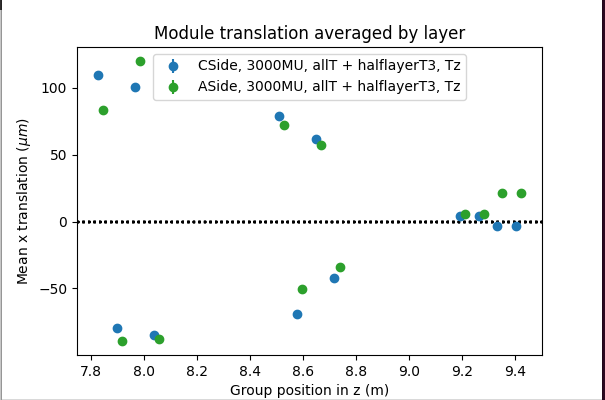
\includegraphics[width=0.8\textwidth]{plots/june_21/CA_allT_halfT3_Tz.png}
  \caption{compare C-Side to A-Side for translation in z direction. (look up exact constraints and dofs)}
  \label{fig:june_5}
\end{figure}

On the other hand the x-translation \ref{fig:june_6}

\begin{figure}
  \centering
  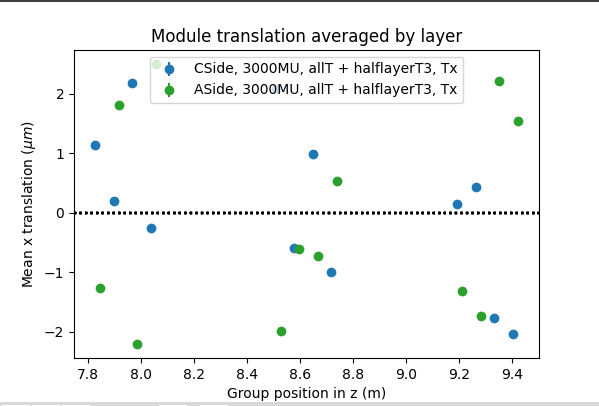
\includegraphics[width=0.8\textwidth]{plots/june_21/CA_allT_halfT3_Tx.png}
  \caption{compare C-Side to A-Side for translation in x direction. (look up exact constraints and dofs)}
  \label{fig:june_6}
\end{figure}

Looking at figure \ref{fig:june_6}, the last two layers in station 3 are
seperation from the first two regarding x-translation. Especially the last
station should be fixed around zero with the constraints added. The sum of
all translations should be zero with each individual layer movement being small.

The result is not what should happen with the constraints added and the cause of this problem is described later.

%\subsection{july plots}
\subsection{rotational constraints}
The impact of rotational constraints is looked at in the followinf chapter. Firstly, comparing
florians starting configuration versus the new one with added constraints.
The direct impact to the rotations are quite small but the translations
in z- and x-direction show a small improvement to the previous configuration
seen in figure \ref{fig:june_4}.

% test 3:
\begin{figure}
  \centering
  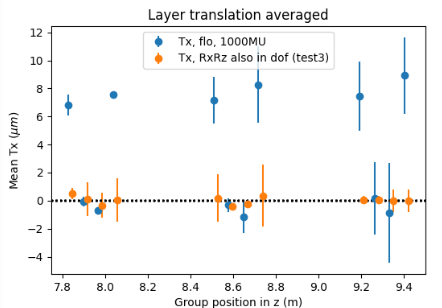
\includegraphics[width=\textwidth]{plots/july_28/Tx.png}
  \caption{Tx versus global z.}
  % \hfill
  % \begin{subfigure}[b]{0.3\textwidth}
  %   \centering
  %   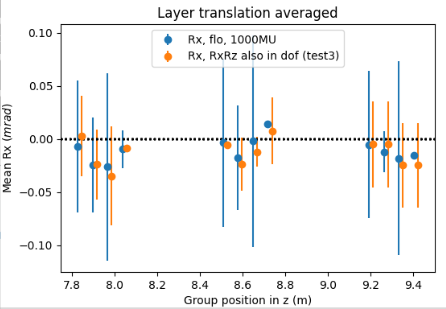
\includegraphics[width=\textwidth]{plots/july_28/Rx.png}
  %   \caption{Rx versus global z.}
  % \end{subfigure}
  % \caption{Testing a configuration versus florians changes.}
\end{figure}

%\subsection{august plots}
% \begin{figure}
%   \centering
%   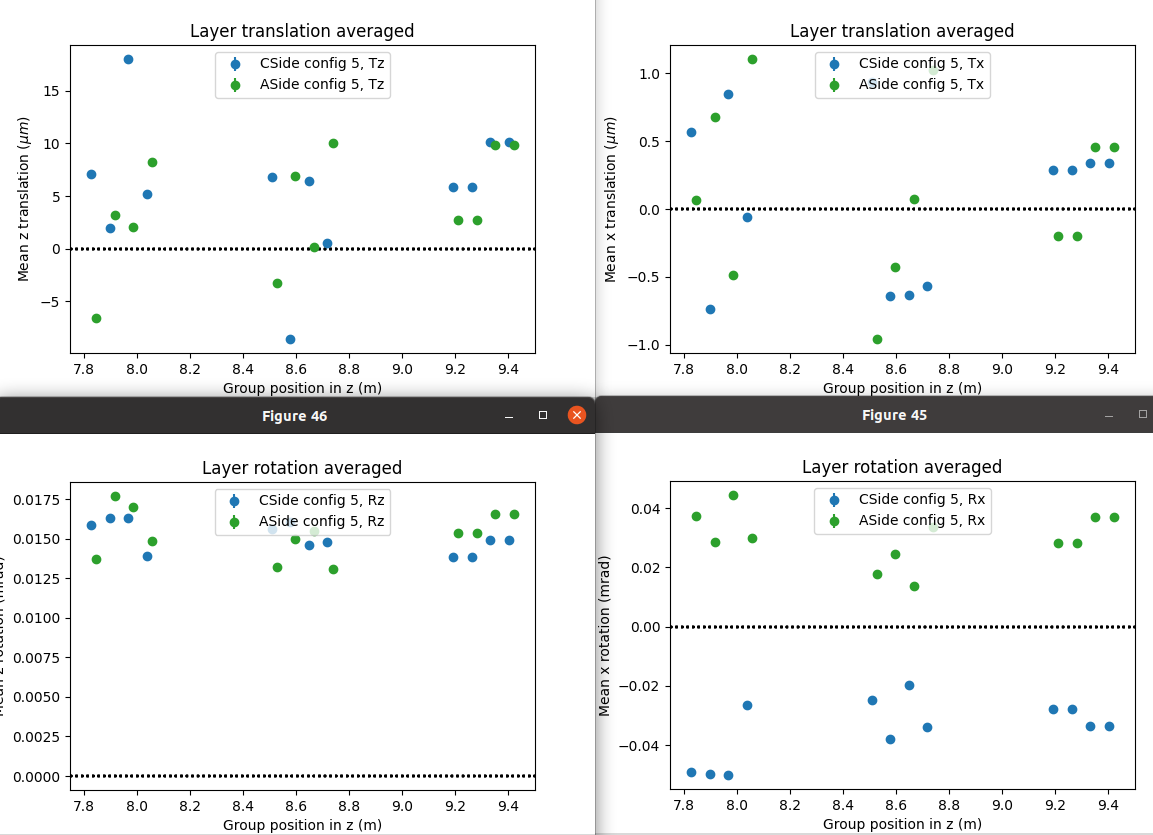
\includegraphics[width=0.8\textwidth]{plots/august_13/C_ASide_config5.png}
%   \caption{old config 5, plotted C and ASide.}
%   \label{fig:aug13_CA_old}
% \end{figure}

% \begin{figure}
%   \centering
%   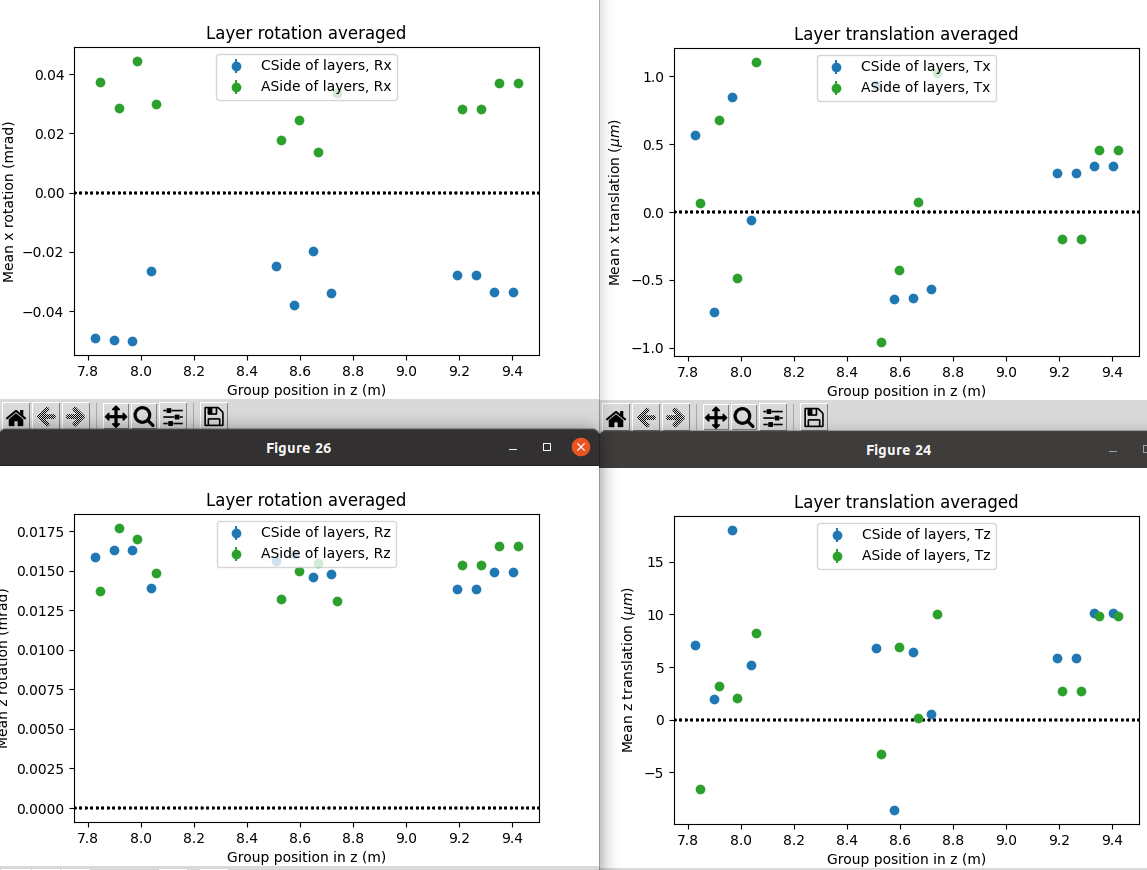
\includegraphics[width=0.8\textwidth]{plots/august_13/CA_side_newconfig5.png}
%   \caption{new config 5, plotted C and ASide.}
%   \label{fig:aug13_CA_new}
% \end{figure}

Now, we have a configuration\footnote{The always used configuration will be
always called "config5" in the labels} which is quite ok but has a lot more room for improvement but is nevertheless a better representation than the first draft from florian.
Therefore we will now compare further configuration drafts to the "config5" with the following constraints
\begin{itemize}
  \item constraint 1
  \item constraint 2
  \item constraint 3
  \item ...
\end{itemize}

and the dataset used is taken from the bookkeeping (which exact one).

\begin{figure}
  \centering
  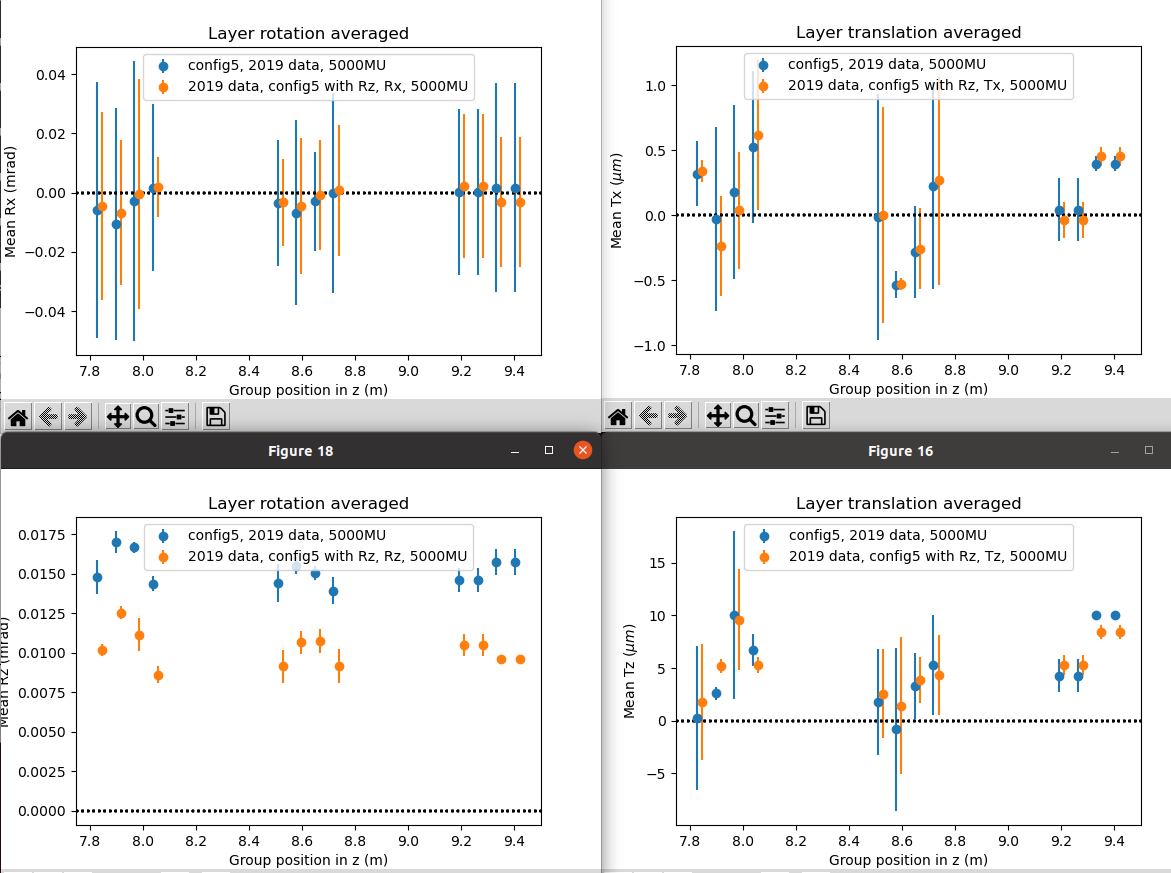
\includegraphics[width=0.8\textwidth]{plots/august_13/2019_c5_old_vs_withRz_MU.png}
  \caption{config5 versus config 5 with Rz constraint for rotational improvement.}
  \label{fig:withRz}
\end{figure}

In figure \ref{fig:withRz} config5 is plotted against itself but with and added constraint to Rz.
The change is the constraint: (fill constraint here).
The result is a small improvement in Rz of around $\SI{0.005}{\milli\radian}$ in every layer. $Rx$ is mostly unchanged and the small differences in $Tx$ are caused by a nudge in the plotting script so that the data points do not overlap. The rotation around $z$ is correlated to the $z$ translation therefore we see small changes in every layer as well.
It is noteworthy, that both X-layers in T2 in the x-translation plot have a quite large RMS uncertainty which means the A-side and the C-side in the X-layers are quite far apart but the mean is right around 0. That is expected since the constraint added only brings the mean of the layer to 0. In future analyses another constraint should be added to also keep the side themselves small.

\begin{figure}
  \centering
  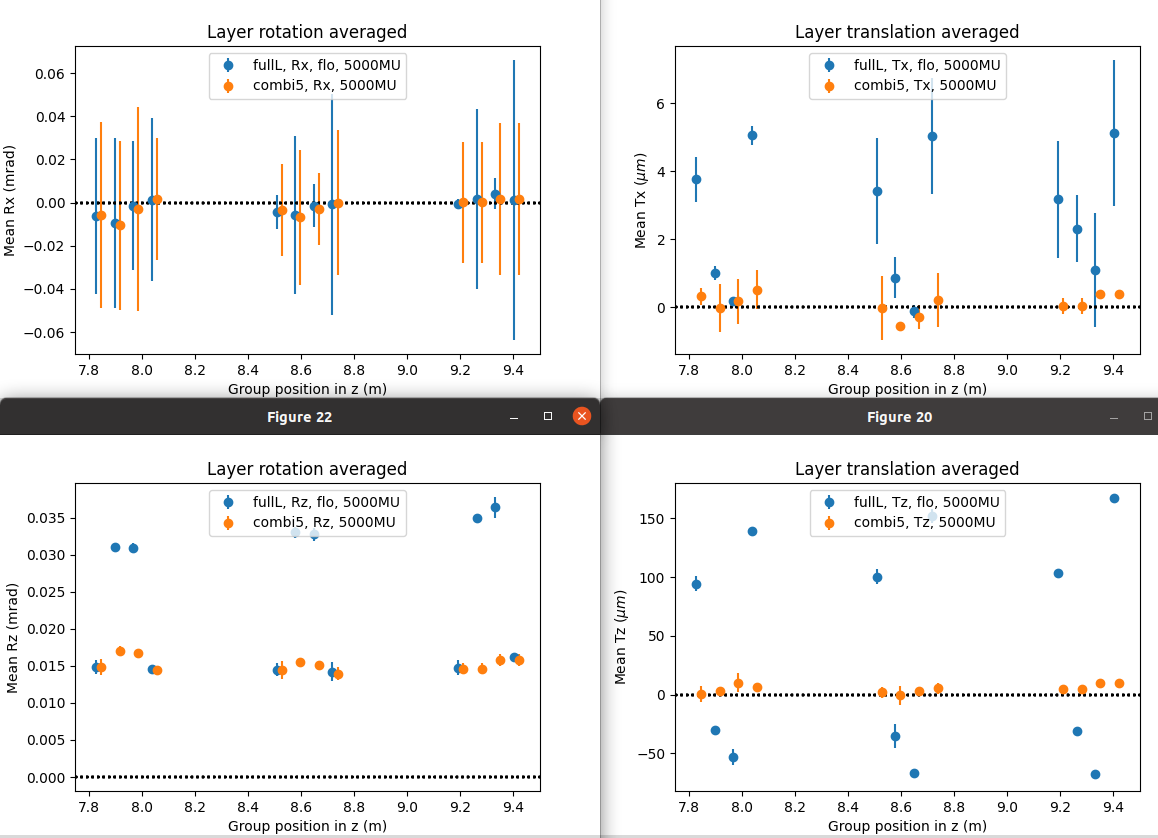
\includegraphics[width=0.8\textwidth]{plots/august_13/combi5_layers_averaged.png}
  \caption{flo with full layer constraint versus config 5}
  \label{fig:floFullL_c5}
\end{figure}

In comparison to what florians configuration looks like against the new
proposed configuration the figure \ref{fig:floFullL_c5} can be looked at.
The alignment was performed for 10 iterations and the alignable degrees of
freedom are $\symup{Tx}, \symup{Tz}, \symup{Rx}, \symup{Rz}$. The alignable
elements are the stations and the framelayers.
The constraints used are: \\
\\
"station3 : FT/T3 : Tx Rz Rx Rz" \\
"backCframeT3 : FT/T3/Layer(V|X2) : Tx Tz" \\
"FT/T3X1UCSide : /dd/Structure/LHCb/AfterMagnetRegion/T/FT/T3/Layer(X1|U)/Quarter(0|2) : Tx Tz Rx Rz" \\
"FT/T3VX2CSide : /dd/Structure/LHCb/AfterMagnetRegion/T/FT/T3/Layer(V|X2)/Quarter(0|2) : Tx Tz Rx Rz" \\
"FT/T3X1UASide : /dd/Structure/LHCb/AfterMagnetRegion/T/FT/T3/Layer(X1|U)/Quarter(1|3) : Tx Tz Rx Rz" \\
"FT/T3VX2ASide : /dd/Structure/LHCb/AfterMagnetRegion/T/FT/T3/Layer(V|X2)/Quarter(1|3) : Tx Tz Rx Rz" \\
\\
The first constraint restricts the overall station 3 movement in $\symup{Tx}, \symup{Tz},
\symup{Rx}$ and $\symup{Rz}$. The second constraint restricts the total movement
of the last C-frame to be 0 but the individual movement can differ.
The last four constraints are C-frame constraints as well but for each halflayer in station 3.

It is good to see that the layer separation in $Rz$ is mostly fixed. But there is still an offset from 0 that is troublesome. This will most certainly have something to do with the clusterbias. Regarding Tx, we have managed to bring down the x-translation to roughly 0 which is a good improvement for the null tests of Tx.

Translation constraints as well as rotation constraints are not the only constraints tested. There are also scaling- and shearing constraints that were analysed but seemed to have
no major impact.

% \begin{figure}
%   \centering
%   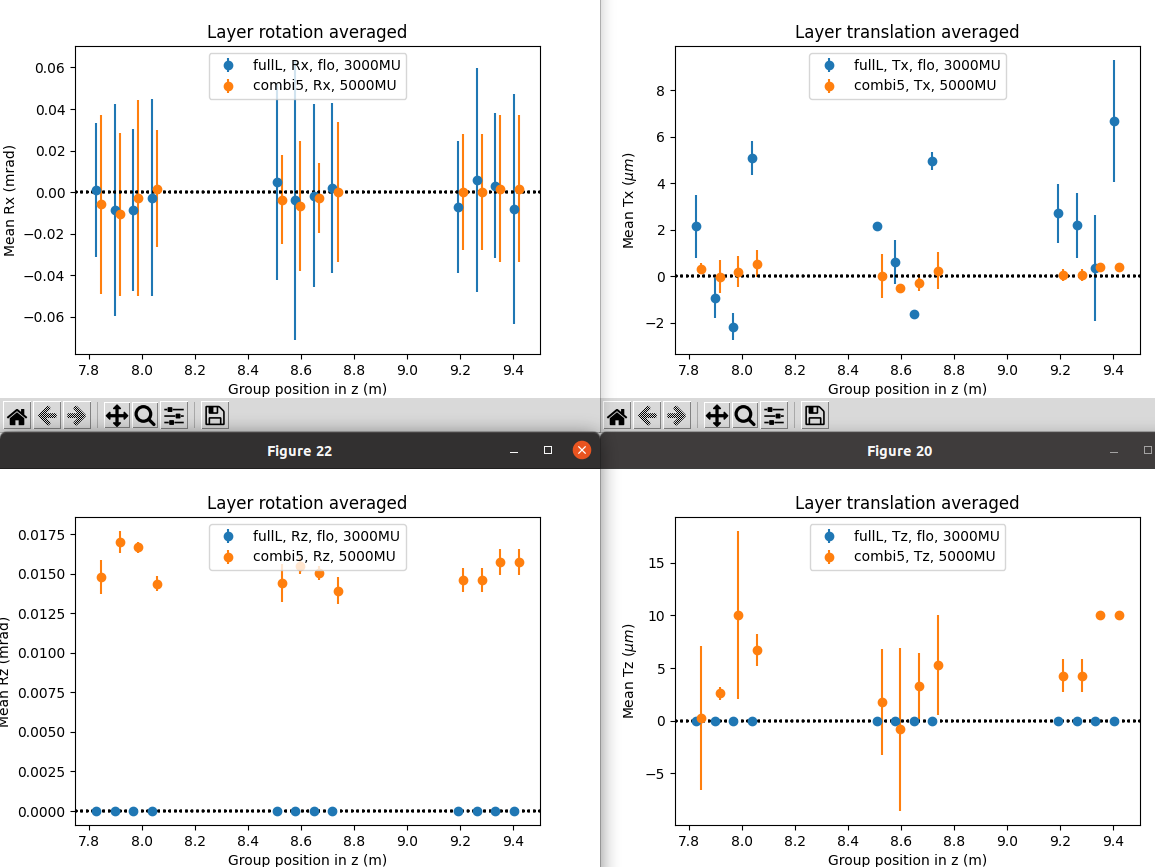
\includegraphics[width=0.8\textwidth]{plots/august_13/newCombi5.png}
%   \caption{original new config 5, should be the first good plot to show!!}
%   \label{fig:OGconfig5}
% \end{figure}
%
% \ref{fig:OGconfig5} only used Tx and Rx as dofs -> bad, dont show this plot (mark for removal)

% october plots
% update: constraining backlayer and also aligning it (append dofs by : Rx Rz)
% Results: \\
% \begin{itemize}
%   \item improves null tests for Rz but not the only reason why its shifted (cluster bias! expand later)
%   \item shearing and scaling constraints do NOT improve this
% \end{itemize}

% Results of 100mu translation misalignment: \\
% 100mu translation misalignment matches expected survey uncertainty. BUT layers shifted from 0 !
% TODO: FTTrackmonitor to study later splitting in track output

\begin{figure}
  \centering
  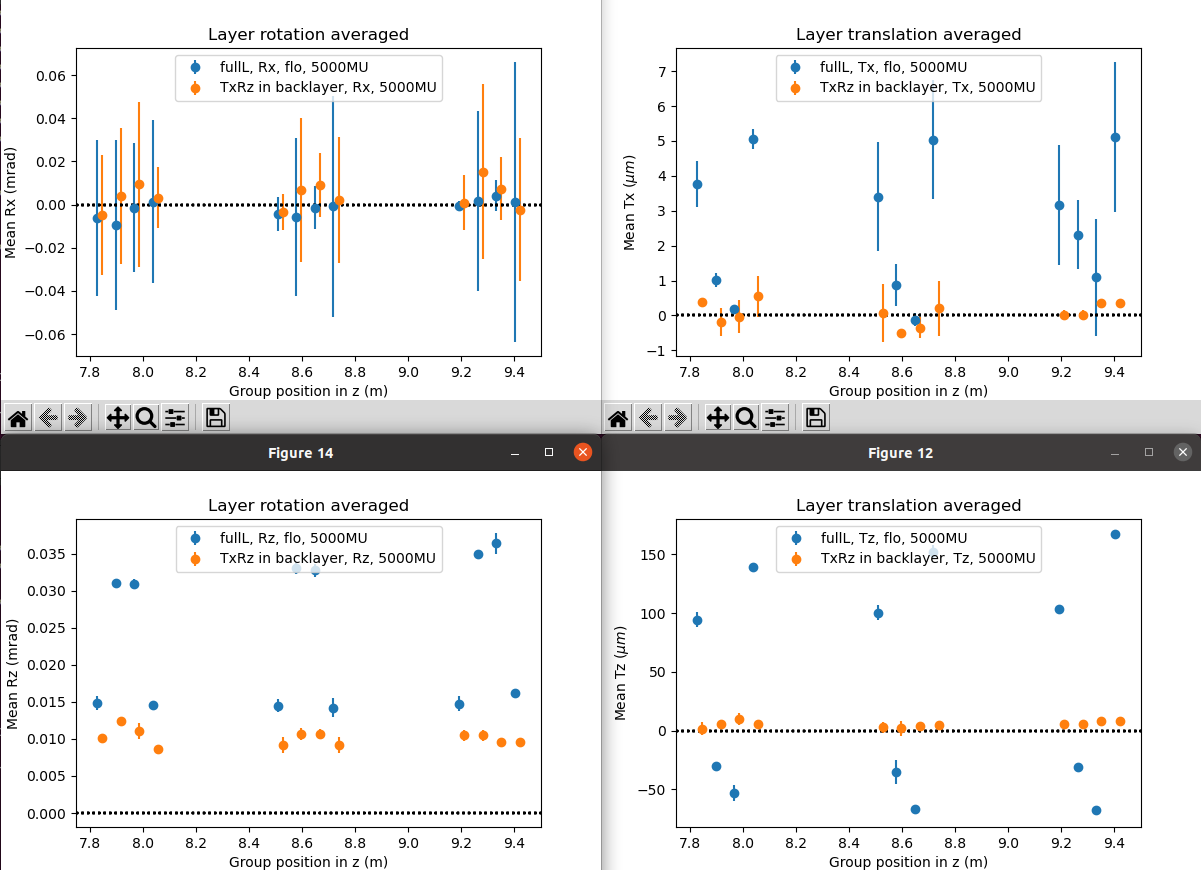
\includegraphics[width=0.8\textwidth]{plots/oct_4/TxRz_config5_backlayer.png}
  \caption{dofs Tx Rz and backlayer constraints.}
  \label{fig:oct4}
\end{figure}

\begin{figure}
  \centering
  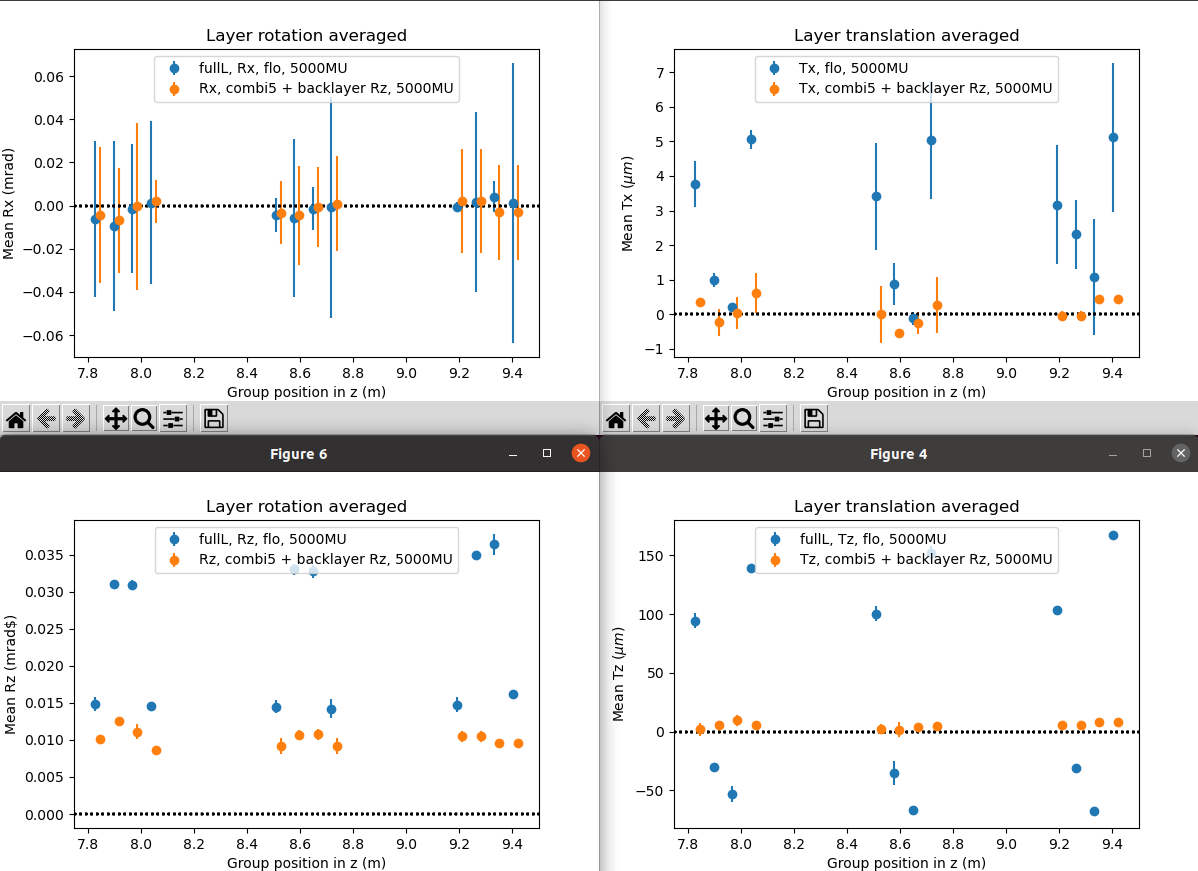
\includegraphics[width=0.8\textwidth]{plots/oct_6/combi5_added_RZ_backlayer.png}
  \caption{combi 5 with Rz backlayer constraint.}
  \label{fig:oct6}
\end{figure}

%TODO: redo the plots for \ref{fig:oct4} and \ref{fig:oct6} and don't use florian
%but instead use a different config5 to compare with!

% november plots
\section{chi2 tests and weak modes}
In this section, a $\chi^2$ analysis is performed in order to study the "goodness" of the alignment since the better the $\chi^2$ after the alignment the better.
The second aspect i want to cover is the impact of potential weak modes also known as "correlated alignment parameters". There are several weak modes that could occur namely \textit{global translation}, \textit{shearing} and \textit{curvature bias}.
Weak modes are unaffected by the $\chi^2$ since the residuals do not change but they do however show inside the eigenvalues of track parameters.
The effect weak modes have on the alignment are biases regarding track parameters and late convergences.
There are different solutions that can be utilized to reduce the effect from weakmodes such as
\begin{itemize}
  \item $\textbf{using other configurations like magnet off or mass plots for off-axis events}$
  \item $\textbf{utilizing other survey data sets}$
  \item $\textbf{using kinematic and vertex constraints}$
\end{itemize}\,.

\begin{figure}
  \centering
  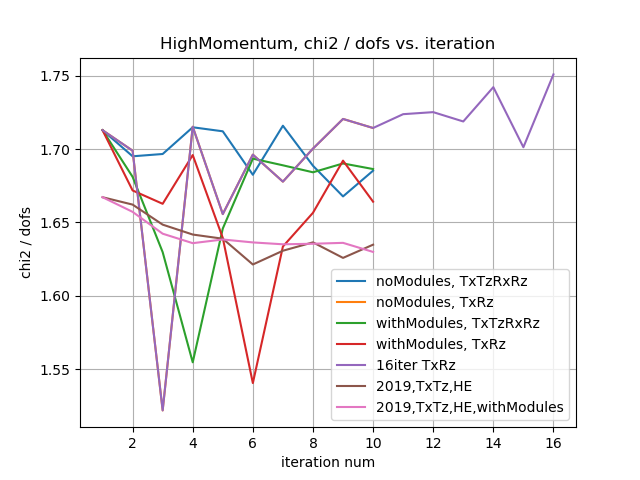
\includegraphics[width=0.8\textwidth]{plots/nov_19/Figure_2.png}
  \caption{$\chi^2 / dofs$ versus iteration number of different degrees of freedom, alignables and data samples.}
  \label{fig:fig2}
\end{figure}

We started with the $\chi^2$-analysis for \textit{HighMomentumTTracks},
6500 events and 2020 data plotted versus the iteration number during the
alignment in figure \ref{fig:fig2}. In blue, stations and layers were aligned in $Tx$,
$Tz$, $Rx$ and $Rz$ with the constraints being used from "config5". The orange
measurement is identical except for the degrees of freedoms being only $Tx$ and $Rz$.
In green and red the same measurements as in blue and orange were performed with
the difference that that the modules are aligned as well.
The purple measurement is the only one which covers 16 iterations and is otherwise identical to the orange one. That is also why the orange measurement is not visible since it lies behind the purple one for the first 10 iterations.
the brown and pink measurements are done for 2019 data and are otherwise identical to the orange and red measurement regarding constraints and alignable degrees of freedom.

The spikey behavior is not what we expected and this might be the result of weak modes since the convergence is quite bad in all of the 2020 data which can be seen by the not
steadily decreasing $\chi^2 / dofs$.
The 2019 measurements were performed as control measurements with and without
module alignment. Here a clear decrease in the $\chi^2 / dofs$ is visible. This
indicates that for the 2020 data additional analysis must be performed to gain further knowledge about the dataset since it shows some unclear findings.

The idea to test $Tx$, $Tz$, $Rx$ and $Rz$ versus only one translation and one
rotational degree of freedom was to analyse the effect regarding the convergence and the $\chi^2 / dofs$ itself. One could also argue that there was a quick convergence after three iterations when looking at the yellow measurement but something happened afterwards. This will be analysed in a future project.

Also, in figure \ref{fig:chi2iter} the same plot is presented but only for the first four measurements clean up the image. The same four $\chi^2$ measurements were plotted
against the number of tracks as seen in figure \ref{fig:chi2tracks}. It is pleasing to see a steady decrease in $\chi^2 / dofs$ with an increasing number of tracks. This was done as a consistency check.

\begin{figure}
  \centering
  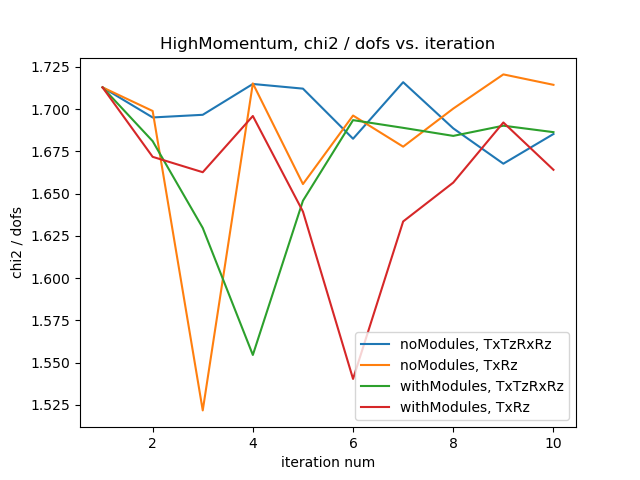
\includegraphics[width=0.8\textwidth]{plots/nov_21/chi2_vs_iter_all.png}
  \caption{$\chi^2$-test versus iteration number of different degrees of freedom, alignables and data samples but fewer (redo with grid).}
  \label{fig:chi2iter}
\end{figure}

\begin{figure}
  \centering
  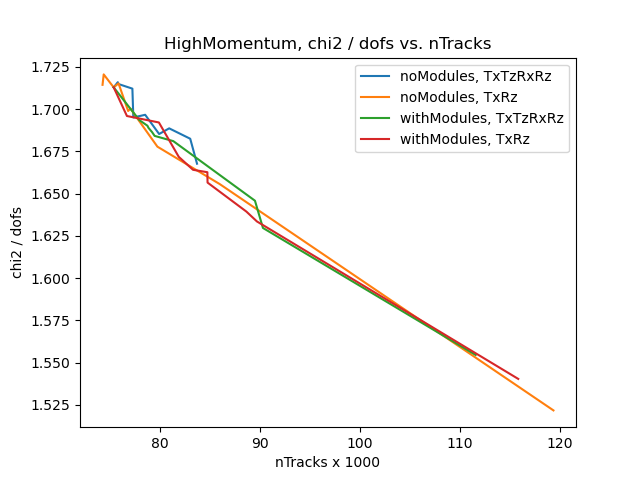
\includegraphics[width=0.8\textwidth]{plots/nov_21/chi2_vs_ntracks_all.png}
  \caption{$\chi^2$-test versus number of tracks of different degrees of freedom, alignables and data samples but fewer (redo with grid).}
  \label{fig:chi2tracks}
\end{figure}

% december plots
\begin{figure}
  \centering
  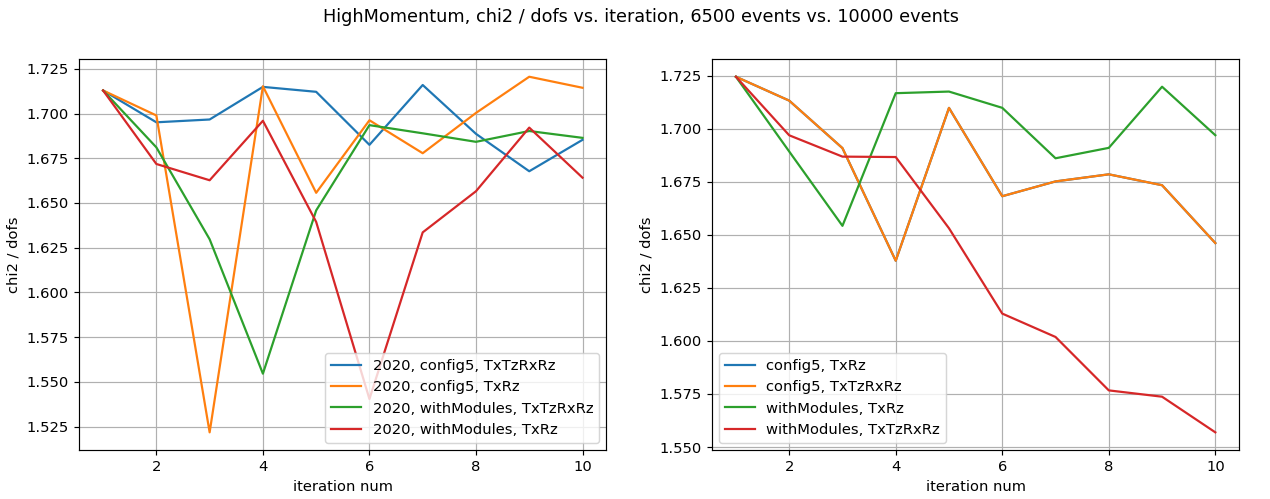
\includegraphics[width=\textwidth]{plots/LHCB_week_dec/chi2_vs_iter_normal.png}
  \caption{$\chi^2 / dofs$ versus iteration number for different number of events.}
  \label{fig:chi2iterdec}
\end{figure}

In figure \ref{fig:chi2iterdec} a side-by-side view of the same $\chi^2$ measurement
is shown but for different number of events. Despite the different labels these are the same measurements, only the colors are switched around for red and green and also yellow and blue as a pair. The thing that strikes the eye is the steadily decrease in $\chi^2 / dofs$ in the red measurement. Unlike our first expectations that $Tx$ and $Rz$ are enough degrees of freedom to describe the system using additional degrees of freedom seemed to help the alignment.
Also, the blue measurement sits behind the orange which might be due to an
programming error.

In figure \ref{fig:chi2tracksdec} a consistency check for figure
\ref{fig:chi2iterdec} was performed. The number of tracks correlate good with
the $\chi^2 / dofs$. The blue measurement is missing again which seems to be a
programming error.

\begin{figure}
  \centering
  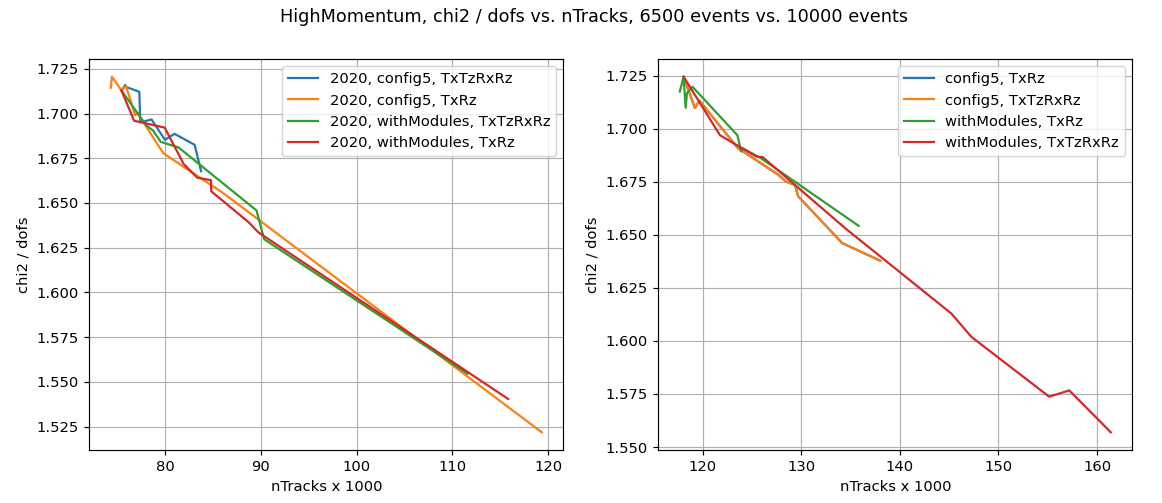
\includegraphics[width=\textwidth]{plots/LHCB_week_dec/chi2_vs_tracks_normal.png}
  \caption{$\chi^2 / dofs$ versus number of Tracks for 6500 events and 10000 events.}
  \label{fig:chi2tracksdec}
\end{figure}

% january plats
% january 17th plots are for luminosity comparisons.
% nu for ramp up luminosity versus lumi during data taking.

\section{luminosity samples and chi2}
For a cross check regarding upcoming studies the difference in $\chi^2 / dofs$ for samples of different luminosities are looked at.
Comparing two samples, one with a "ramp-up" luminosity with a parameter $\nu = 3.8$ also referred to as "low luminosity" and one for the luminosity used during the data taking
with $\nu = 7.6$, called "normal luminosity".
Plotted are these samples in $\chi^2 / dofs$ versus the iteration number \ref{fig:chi2iter_lumi_normal} and the number of tracks\ref{fig:chi2tracks_lumi_normal}.

in figure \ref{fig:chi2iter_lumi_normal} we see the expected convergence after iteration three and a quite low $\chi^2 / dofs$ of around $\num{1.28595}$ for the normal luminosity sample
and $\num{1.3067}$ for the low luminosity sample.

\begin{figure}
  \centering
  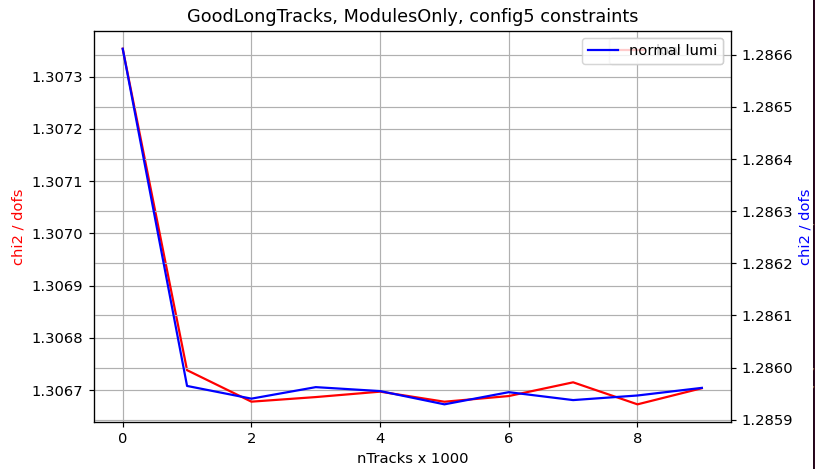
\includegraphics[width=0.8\textwidth]{plots/jan_17_2022/chi2_iter_low_vs_normal.png}
  \caption{compare different luminosities and plot $\chi^2$ versus iteration.}
  \label{fig:chi2iter_lumi_normal}
\end{figure}

%for figure \ref{fig:chi2iter_lumi_normal} redo the plot with correct labels and legend !!

\begin{figure}
  \centering
  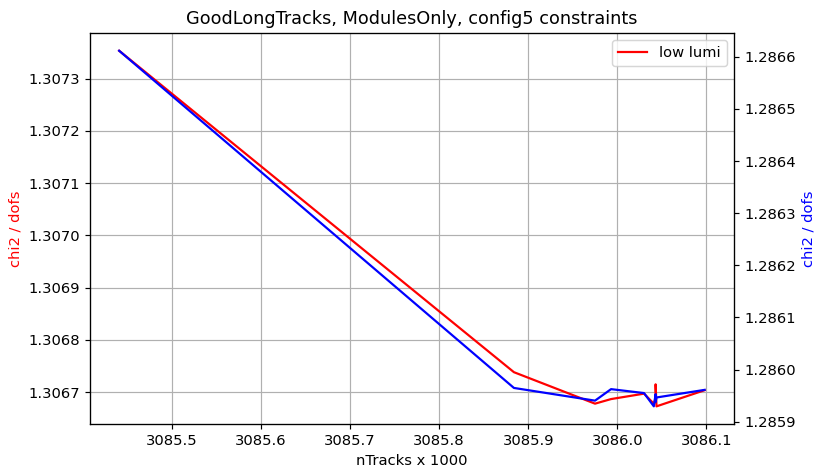
\includegraphics[width=0.8\textwidth]{plots/jan_17_2022/chi2_tracks_modulesOnly.png}
  \caption{compare different luminosities and plot chi2 versus number of tracks as a measurement for weakmodes and alignment.}
  \label{fig:chi2tracks_lumi_normal}
\end{figure}

% \begin{figure}
%   \centering
%   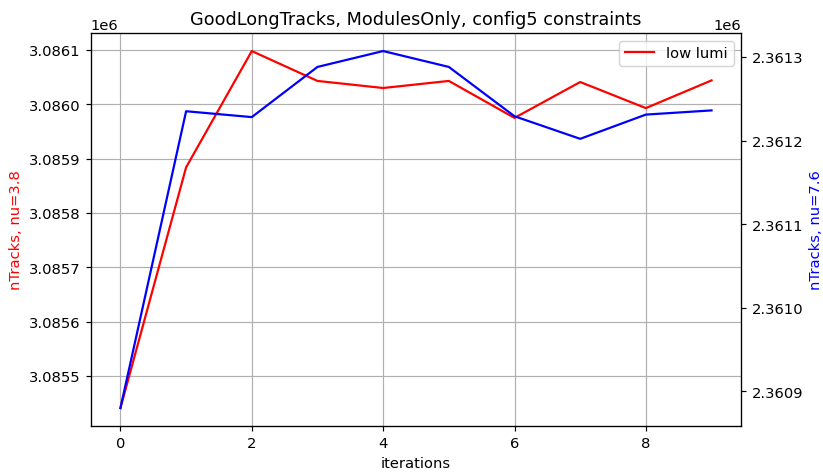
\includegraphics[width=0.8\textwidth]{plots/jan_17_2022/tracks_vs_iterations_modulesOnly.png}
%   \caption{compare different luminosities and plot number of tracks versus iteration number as a measurement for weakmodes and alignment.}
%   \label{fig:chi2iter_lumi_normal}
% \end{figure}

% january 24th:
\section{impact of the cluster bias}

As mentioned earlier the clusterbias most certainly causes the shift in the rotation around z for each layer so it does not reach 0.
To test that a momentary fix was found and implemented. The workaround was to a add a scaling to the value ... (look up in LXPLUS) by $\num{0.95}$.

Figure \ref{fig:cbhack_on_off} shows the impact of the cluster bias hack regarding
the rotation around $z$.

% show that there is a visible difference between low and normal luminosity however the difference is not big enough to differentiate between the two phases during the ramp up and full run. therefore, for the upcoming analysis steps only the "normal/low" luminosity is taken into consideration.

\begin{figure}
  \centering
  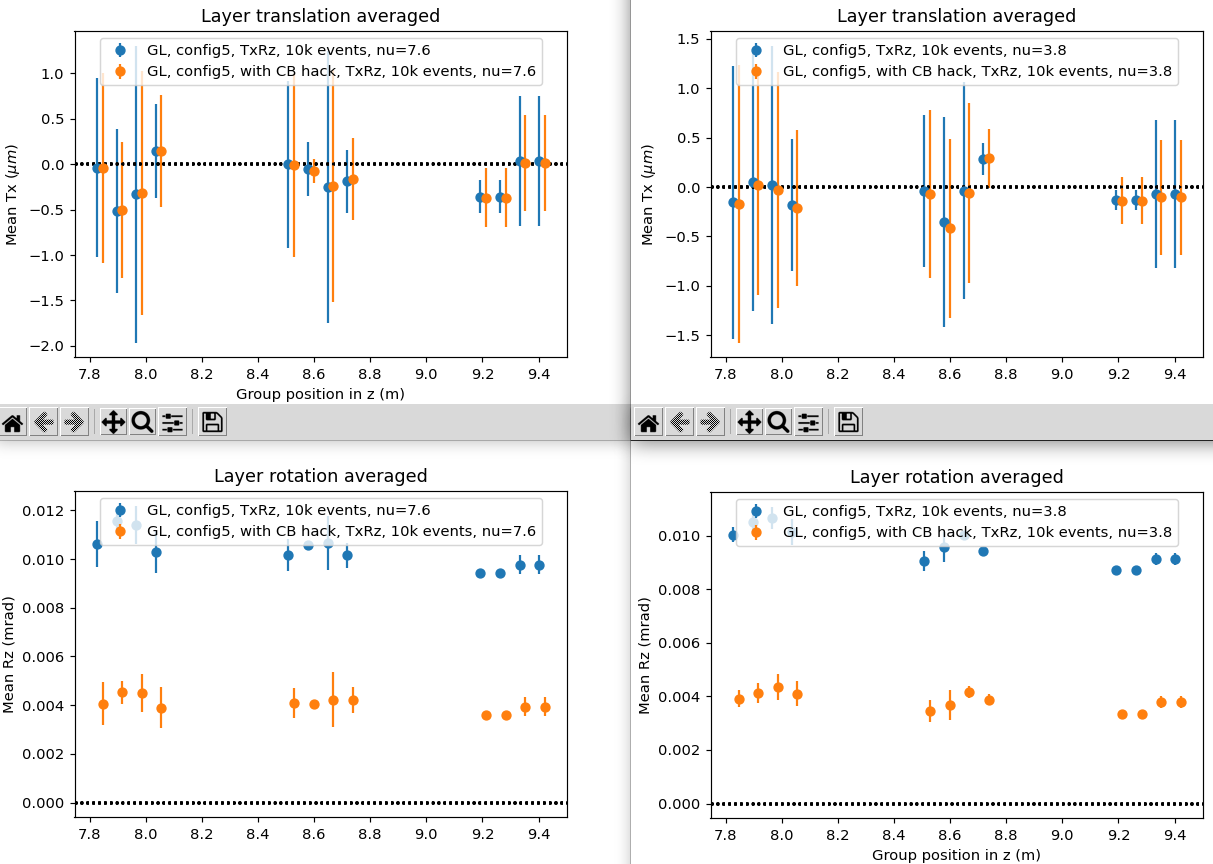
\includegraphics[width=0.8\textwidth]{plots/jan_24_2022/compare_with_without_hack.png}
  \caption{Impact of the clusterbias betweenfor high and low luminosity samples.}
  \label{fig:cbhack_on_off}
\end{figure}

As we expected, the amount of rotation was reduced to about
$\SI{0.004}{\milli\radian}$ from the previous $\SI{0.01}{\milli\radian}$ which is more than a factor of 2 improvement. We also know, that the fix for the cluster bias will not be the only source for the shift and we need further analysis to find the other sources.

Now that we know that the cluster bias can be taken care of we take a closer look at samples of different luminosities since the LHC will not be operated at the maximum luminosity from the start, there is also the ramp up phase where the luminosity will be lower.

Since we want to know what the shifts in rotation and translation will look like when the cluster bias is fixed we will keep it active for the next studies.
Figure \ref{fig:lumi_low_normal_hack_on} shows the difference between a sample with ramp-up luminosity and a sample with the luminosity during the measurement phase.
We see, that the layer separation is much more prominent in station 1 and 3 for the higher luminosity sample but slightly better behaved in station 2 when looking at x-translation.
Regarding the z-rotation, the lower luminosity sample as slightly lower rotational shifts.
The difference is so minute that it can be safely disregarded. (not sure about that)

\begin{figure}
  \centering
  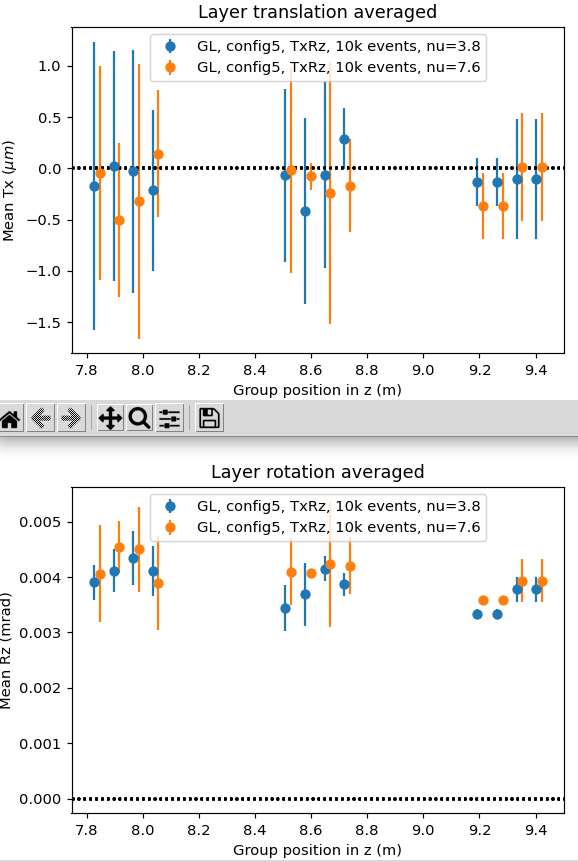
\includegraphics[width=0.8\textwidth]{plots/jan_24_2022/low_normal_with_hack.png}
  \caption{show difference between low and normal luminosity with clusterbias hack active.}
  \label{fig:lumi_low_normal_hack_on}
\end{figure}

% february plots
With that, we tested if there is a noticable difference in the $\frac{\chi^2}{\text{dof}}$
and the result is shown in figure \ref{fig:GL_lumi_low_normal_hack_on}.
% The scale is a little bit confusing so i will redo this plot for better readability.

\begin{figure}
  \centering
  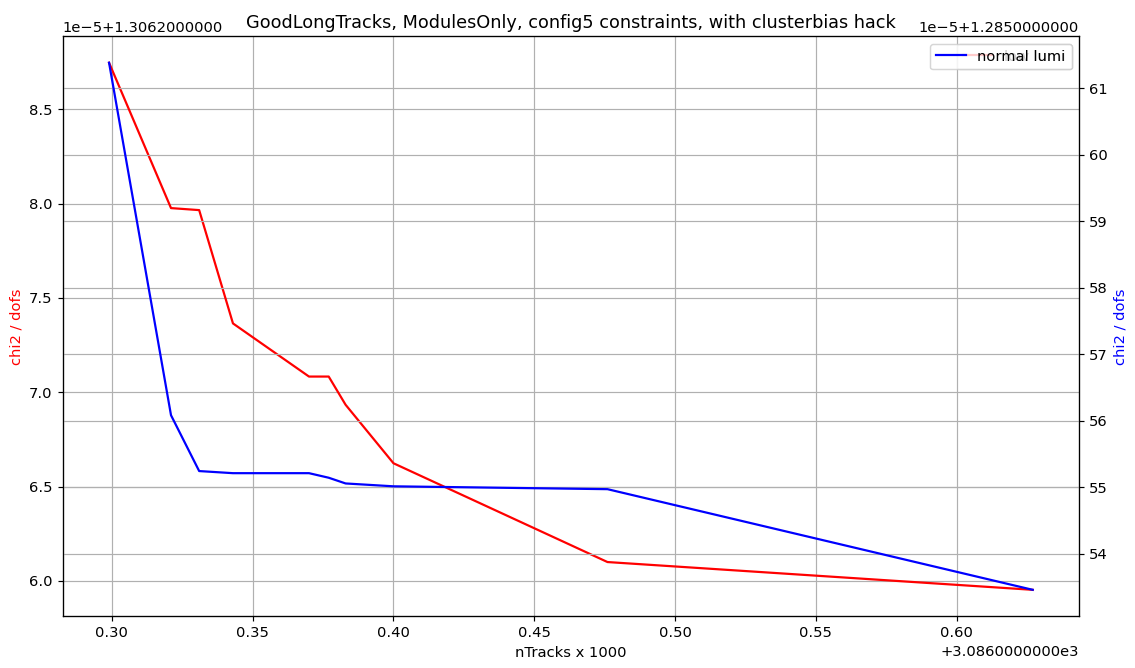
\includegraphics[width=0.8\textwidth]{plots/feb_2_2022/GL_modules_c5_cb_hackactive_low_normal_lumi.png}
  \caption{GoodLong tracks for module alignment and config 5 active. also the clusterbias hack is active comparing low and normal luminosity.}
  \label{fig:GL_lumi_low_normal_hack_on}
\end{figure}

\begin{figure}
  \centering
  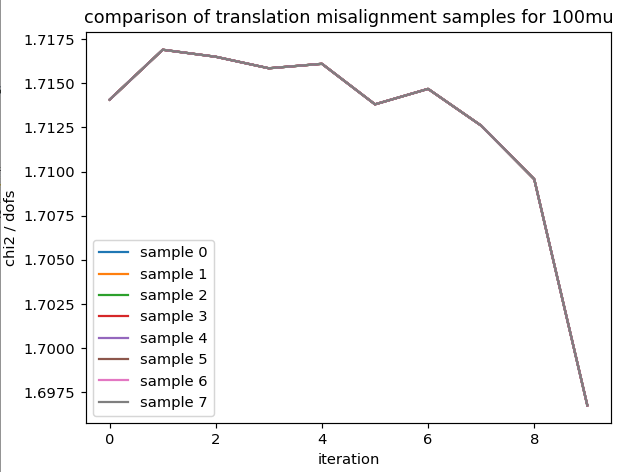
\includegraphics[width=0.8\textwidth]{plots/feb_6_2022/100mu_misalignment_samples_compared.png}
  \caption{100mu translation misalignment comparison for different misalignment samples.}
  \label{fig:100muT}
\end{figure}

Now, since the alignment works quite good with the current configuration we
tested how translation misalignment effects the convergence by looking at the
$\chi^2$, portrayed in figure \ref{fig:100muT}. For this figure, eight different samples of $\SI{100}{\micro\metre}$ module translation misalignment over all translatory
degrees of freedom. The idea behind using different samples is to reduce errors
from biased samples. The plot shows the total $\chi^2$ over degrees of freedom
plotted against the number of iterations. We see no visible difference regarding
the total $\chi^2$ between the samples which is good.
Also, the total $\chi^2$ decreases with an increasing number of iterations
during the alignment.

\begin{figure}
  \centering
  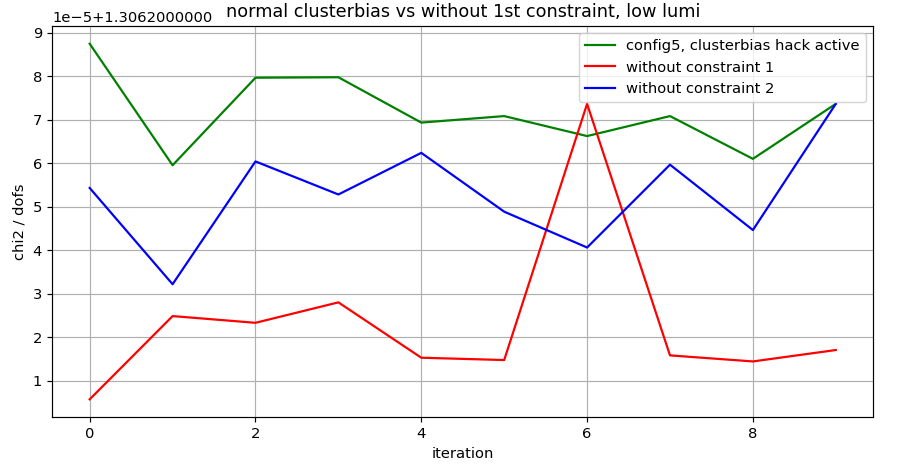
\includegraphics[width=0.8\textwidth]{plots/feb_6_2022/low_lumi_removed_constraints_vs_normal.png}
  \caption{impact of removing constraints from exisiting studies regarding chi2.}
  \label{fig:removeConst}
\end{figure}

We do want the least amount of constraints in the system so we also tested
the consequences of removing constraints from "config5".
The results are shown in figure \ref{fig:removeConst}.
The green curve shows the base config for comparison and in red the removal of the backlayer constraint in station 3 is shown. The blue curve shows the alignment results without the C-frame constraints.
The data samples used were from 2020 with the normal luminosity and an active clusterbias hack.
The selected track types are \textit{HighMomentumTTracks}(?) for 10000 events (?).
On the one hand we see an improvement in $\chi^2 / \text{dof}$ when removing these constraints individually even if it is only on a very small scale of $\num{1e-5}$. On the
other hand we see that the $\chi^2 / \text{dof}$ after the last iteration is the same for the base config and for the blue measurement. The constraint removed in the red measurement seems to have the most impact from what was tested but the peak in iteration 6 has no logical
explanation for now. Additional analysis regarding constraint removal will be done in the future to analyse this phenomenon further.
Also the behavior of the not decreasing $\chi^2 / \text{dof}$ requires more testing.
What can be taken from this is that the removal of some constraints will help
the alignment but the cause of some abnormalities require more testing.
